%------------------------------------------------------------------------------
% This is a LaTeX template for the scientific justification of IRAM Proposals 
%------------------------------------------------------------------------------
% 
% We encourage IRAM proposers to use this template for the sake of unity 
% and clarity when Program Committee members assess their proposals.
% 
% You may customize this template to suit your preferences (e.g. using BibTex),
% but please respect the following requirements:
%     The scientific justification should contain a maximum of 2 pages of text 
%     (4 pages for Large Programs), plus 2 pages of Figs., Tables and Refs.
%     The font size should be 11pt or larger.
%
% For Large Programs, the following sections should be included: 
%   i) Scientific Rationale, 
%  ii) Immediate Objective, 
% iii) Feasibility and Technical Justification, and 
%  iv) Organizational Issues.
% 
%
%------------------------------------------------------------------------------
%
\documentclass[11pt,a4paper,twoside,graphicx,color]{article}
%
\usepackage[margin=2cm]{geometry}
\usepackage[pdftex]{graphicx}
\usepackage{color}
\usepackage{txfonts}
\usepackage{paralist}
\usepackage[numbers]{natbib}
\setlength{\bibsep}{0.0pt}
\usepackage{amssymb}

\newcommand{\ccor}[1]{\textcolor{red}{#1}}

%
% Page size and text dimensions
% Do not change!
\textheight 260mm
\textwidth 178mm
\oddsidemargin -8mm
\evensidemargin -8mm
\marginparwidth 50pt
\topmargin -22mm
\brokenpenalty=10000
\sloppy
%
%-------------------------------------------------------------------
\begin{document}
%
%
\begin{center}{\huge \bf
%-------------------------------------------------------------------
Sunyaev-Zel'dovich follow up of relaxed high redshift Planck galaxy clusters (NIKA GT)
%-------------------------------------------------------------------
}\end{center}
% 
\centerline{\bf P.I.: B. Comis,  R. Adam \& G.W. Pratt}

%---------- Abstract to be put on the web
%We aim to observe {\bf three high redshift ($z > 0.5$) clusters of galaxies} recently discovered by the Planck satellite via the {\bf thermal Sunyaev--Zel'dovich} (tSZ) effect and for which X-ray follow-up observations indicate relaxed morphologies. The NIKA data will constrain the ICM  morphology and provide pressure profiles out to about 3 arcmin. Combination with XMM (X-ray) observations will yield further insights into the ICM thermodynamics and allow comparison of X-ray and SZ-derived quantities such as SZ signal $Y_{\rm SZ}$, its X-ray analogue Y$_{\rm X}$, and pressure.  Together with our recent NIKA observations of three merging systems, these data will allow us to sample a representative range of ICM morphology (relaxed, disturbed) and $Y_{\rm SZ}$ for Planck-detected systems. The full sample of six objects will constitute a pilot study to prepare for a Large NIKA2 Program to observe Planck SZ-detected clusters of galaxies via the tSZ effect.

%%%These observations %will be done with the NIKA camera and will be will be a pilot study in order to {\bf prepare the Large NIKA2 Program for observing cluster of galaxies via the tSZ effect}. The obtained NIKA data will be combined with Planck and XMM (X-ray) observations to constrain the {\bf morphology}, and {\bf thermodynamic properties} of the clusters, and to derive physical parameters such as their masses. We will use $6 \times 3$ arcmin OTF scans. We will consider mainly the 150 GHz channel and we ask for an opacity at 225 GHz lower than 0.17 (less than 4 mm of precipitable water vapor). The total requested observing time is {\bf 30 hours} in order to reach a RMS of about 0.3 mJy/beam for each cluster at the tSZ peak.

%-------------------------------------------------------------------
\vspace{-0.3cm}
\section{Scientific context}
\vspace{-0.3cm}
{\bf \large Introduction -- } 
Clusters of galaxies provide valuable information concerning the evolution of the Universe and the {\bf formation of large scale structures} \cite{planck_cluster_count2013}. Their observable properties reflect their formation through hierarchical gravitational collapse. However, non-gravitational processes such as feedback from AGN and supernova-driven galactic winds can alter these observed properties to a large extent. Consequently a detailed characterization of the complex interplay between the gravitational and non-gravitational processes acting on clusters is mandatory for a detailed {\bf understanding of their astrophysics}. This is in turn essential for their use as {\bf cosmological probes}.%in order to properly use them as a strong cosmological probes.

%However, in the case of disturbed systems, their physics is often complex and not well understood, in particular at the substructure level. Consequently a detailed characterization of the complex gravitational and non-gravitational processes acting on clusters is mandatory not only for a detailed understanding of their astrophysics, but also in order to properly use them as a strong cosmological probes.

Most of the cluster baryons are in the form of a hot ionized gas, constituting the intra-cluster medium (ICM). They are responsible for the Bremsstrahlung {\bf \mbox{X-ray} emission}, related to the electron density and temperature along the line of sight ($S_X \propto \int \sqrt{T_e} n_e dl$, see \cite{bohringer2010} for a detailed review). On the other hand, {\bf the thermal Sunyaev-Zel'dovich (tSZ) effect} is a distortion of the black body CMB (Cosmic Microwave Background) spectrum produced by the inverse Compton interaction of CMB photons with the hot electrons of the ICM \cite{sunyaev1972,sunyaev1980}. After this interaction a fraction of CMB photons is moved to higher energies, with a resulting flux decrement ({\it resp.} increment) at frequencies below ({\it resp.} above) the null point at 217 GHz. The tSZ effect amplitude is given by the Comptonization parameter, proportional to the integral of the {\bf electron pressure} along the line of sight ($y \propto \int P_e dl$). The integrated Compton parameter up to a given radius $\theta_{\mathrm{max}}$, $Y_{\theta_{\mathrm{max}}} = \int_{\Omega(\theta_{\mathrm{max}})} y\, d\Omega$, is then directly related to the {\bf cluster thermal energy and its mass}. See \cite{birkinshaw1999} for a detailed review on the tSZ effect. Numerical simulations indicate that the spherically-integrated tSZ effect correlates particularly strongly with the total mass \cite{das04}, making it a valuable tool for assembly of samples that are as near as possible to mass-selected. Furthermore, since the observable is the spectral distortion of the CMB, the tSZ effect is in principle a redshift independent probe of the pressure of the electron population that produced it. 

Observations through the tSZ effect are now providing a reliable tool to push cluster detection and characterization to higher redshifts. In particular, tSZ surveys by Planck, SPT, and ACT have proved to be very complementary to traditional methods of cluster detection ({\it e.g.} X-ray, optical), and have contributed to a substantial increase in the number of high redshift ($z>0.5$) clusters known. In this context, full sky tSZ measurements by the Planck satellite \cite{planck_sz_cat2013, planck_ymap2013} have proved to be very competitive, since the large volume of the Planck survey allows the rarest, most massive clusters to be found. However, Planck's relatively poor angular resolution ($\sim$ 5', \cite{planck_overview2013}) means that follow-up with dedicated instruments with much {\bf higher angular resolution is required} in order to better address the physics at play, especially when dealing with intermediate and {\bf high redshift objects}. Furthermore, the use of a sample of tSZ-selected objects for cosmology requires the understanding of how matter is distributed and the evaluation of the scatter that different systems may introduce in the tSZ flux-to-total mass relation. High resolution measurements of cluster pressure profiles, impossible with Planck except for nearby objects, are a mandatory step towards this goal. \\

\vspace{-0.3cm} \noindent {\bf \large Previous observations with NIKA -- }  
Ground-based observations of galaxy clusters may suffer from large angular scale filtering due to atmospheric noise removal. {\bf Dual-band observations} can be used to remove the atmospheric noise without affecting the signal, taking advantage of the characteristic tSZ spectrum. Indeed, while the tSZ signal is negative at 150 GHz and positive in the 260 GHz band, the atmospheric noise is roughly proportional to $\nu^2$. This allows to combine the two bands in order to extract the tSZ signal at 150 GHz (see \cite{adam2013} for technical details). In this context, NIKA appears as a well-adapted instrument for high-resolution tSZ observations, being able to recover {\bf both small angular scales} (down to about 20", limited by the beam) {\bf and large angular scales} (up to the scan size, $\sim$ 300").  

We have observed a small sample of 3 Planck-detected clusters as part of NIKA run 5 and first NIKA pool. The objects were chosen as they were well-known in X-ray and were predicted to yield a strong tSZ signal. As shown in Fig.~\ref{fig:clusterRun8}, NIKA is capable of producing high-quality maps with excellent angular resolution ($\sim 20"$), enabling detailed examination of cluster morphology through the tSZ effect. Furthermore, as shown in the deep observation of \mbox{RX~J1347.5-1145} in \cite{adam2013}, combination with X-ray observations yields additional information, such as the location of shock-heated regions of the ICM. Moreover, these data afford pressure profile measurements on angular scales (tens of arcsec) that are complementary to, and indeed competitive with those available from X-rays. Combination of these high-resolution tSZ observations with X-ray data presents a uniquely powerful tool to investigate these systems.\\

\vspace{-0.3cm} \noindent {\bf \large Proposed observations -- }
Here we propose to observe {\bf three high-redshift} ($z > 0.5$) Planck tSZ-detected clusters of galaxies as part of a {\bf NIKA2 pilot study}. In combination with the previous observations described above, these data will allow us to sample a representative range of cluster X-ray morphologies and test NIKA detection at lower tSZ signals and Planck detection significance. All clusters have rich ancillary data sets, such as X-ray observations obtained with XMM (as part of a Large Programme to study Planck clusters at $z>0.5$, PI M. Arnaud) and optical observations obtained with VLT or Subaru.  

%A tSZ dedicated NIKA2 guaranteed time large program is under preparation, and that is why we propose to perform a pilot study with NIKA.
%
%
%and that is why we propose to perform a pilot study with NIKA.
%



%(tens of arcseconds, as it is the case for NIKA) 

%, meaning less virialized objects and non-trivial morphologies. Recent full sky tSZ measurements by the Planck satellite \cite{planck_sz_cat2013, planck_ymap2013} have been proved to be very competitive and complementary to traditional observations of galaxy clusters ({\it e.g.} X-ray, optical). Nevertheless, its relatively poor angular resolution ($\sim$ 5 arcminute, \cite{planck_overview2013}) requires follow-ups with dedicated instruments having much higher angular resolutions (tens of arcseconds, as it is the case for NIKA) in order to better address the physics at play when dealing with intermediate and high redshift objects.

%-------------------------------------------------------------------
\section{Technical justification}
\vspace{-0.3cm}
{\bf \large Target selection -- }
We have selected three clusters of galaxies, PSZ1~G045.85+57.71, PSZ1~G155.25-68.42 and PSZ1~G046.13+30.75 (sorted by order of priority). A brief description of them is given in Tab.~\ref{tab:list_gc}. They have been selected according to the following criteria:
{\bf (1)} -- Recently discovered by the Planck satellite and confirmed to be {\it bona fide} clusters with \mbox{X-ray} follow-up. 
{\bf (2)} -- Redshift larger than 0.5 to ensure an angular size adapted to the NIKA field of view. 
{\bf (3)} -- Large expected tSZ signal. Their integrated Compton parameter, up to a radius within which their mean density is 500 times the critical density of the Universe at the corresponding redshift is respectively $Y_{500} \simeq$ (0.82, 1.03 and 0.77) $\times 10^{-3}$ arcmin$^2$. In comparison, the cluster \mbox{RX~J1347.5-1145} (z=0.45) observed during the NIKA technical run of November 2012 has $Y_{500} = 1.77 \pm 0.32$ arcmin$^2$ and peak at about 10 mJy/beam at 140 GHz (see left panel of Fig.~\ref{fig:clusterRun8} and \cite{adam2013}). We therefore estimate the tSZ signal to peak at about 5, 6 and 4 mJy/beam respectively, assuming a similar flux distribution. 
{\bf (4)} -- Good visibility during the observation period. 
{\bf (5)} -- Circular, centrally-peaked X-ray morphologies indicative of dynamically relaxed systems (see Fig.~\ref{fig:xray}) , in contrast to the unrelaxed morphologies of the systems thus-far observed with NIKA, thus allowing us to probe different dynamical states.
As expected for clusters detected by Planck, all objects are very massive ($M_{500} > 5 \times 10^{14}$ M$_{\odot}$).\\

\vspace{-0.3cm} \noindent {\bf \large Immediate outputs -- }
The aim of our project is the detection and the characterization of the tSZ signal in 1D (profile) and 2D (map) up to $\sim 3$ arcminute. We will:
{{\bf (1)} -- Test the tSZ morphology of the clusters. While these clusters appear relaxed in X-rays, recall that tSZ observations of RX\,J1347.5-11.45, long assumed from X-ray observations to be a prototypical relaxed object, were the first to indicate that the object is undergoing a spectacular merger \cite{poi99,kom99}. 
{\bf (2)} -- Extract the thermal pressure distribution using a high-resolution tSZ flux profile (see, e.g., \cite{adam2013}). This will be compared to that derived from XMM X-ray observations. The two measurements combined can be used to derive independent constraints: for example, the tSZ pressure profile combined with the X-ray density profile can be used to infer an independent  temperature profile, which can be compared to that derived directly from the X-ray data (see e.g., \cite{bas10}). Due to the different dependencies of the X-ray and tSZ signal on the gas density, this type of analysis is a powerful probe of the effect of temperature and density inhomogeneities (gas clumping), but has not been attempted in clusters at $z>0.5$. 
{\bf (3)} -- Derive the global tSZ signal $Y_{\rm SZ}$ and compare to its X-ray analogue $Y_{\rm X} = M_{\rm gas}\times T_{\rm X}$, and the X-ray luminosity $L_{\rm X}$. Using the total mass derived from X-rays (assuming hydrostatic equilibrium) or lensing (derived from Subaru or VLT data), we will also be able to constrain the normalization of the $Y_{\rm SZ}$ -- mass relation at $z>0.5$. Combining these data with existing measurements at lower redshift, we will be able to probe for evolution in these scaling relations. 
%Combine with X-ray observations and derive other quantities such as the gas mass and entropy. Using the total mass derived from X-rays (assuming hydrostatic equilibrium) or lensing (derived from Subaru or VLT data),} the gas mass fraction can be derived. This will allow us to make a first measurement of the range of pressure and entropy profiles in massive clusters at $z>0.5$, and to search for evolution effects in the relations between  $Y_{\rm SZ}$, its X-ray analogue $Y_{\rm X} = M_{\rm gas}\times T_{\rm X}$, the X-ray luminosity $L_{\rm X}$, and the mass. }
{\bf (4)} -- Prepare the tSZ large program with NIKA2 camera that is well adapted for a systematic follow-up of Planck tSZ-detected clusters of galaxies.\\
%Combining the NIKA data with Planck and XMM observations, we will be able to: 
%{\bf (1)} -- Test the tSZ morphology of the clusters. 
%{\bf (2)} -- Extract the thermal pressure distribution and derive other quantities such as the gas mass, the total mass \ccor{(assuming hydrostatic equilibrium), and} the gas fraction. 
%{\bf (3)} -- Search for evolution signatures related to formation processes, accretion and feedback. 
%{\bf (4)} -- Prepare the tSZ large program with NIKA2. 
%\textcolor{red}{c'est en gros le mail d'Etienne mais modifiez comme bon vous semble svp}
%
%\paragraph{Dual-band analysis}
%Ground-based observations of galaxy clusters may suffer from large angular scale filtering due to atmospheric noise removal. Dual-band observations can be used to remove the atmospheric noise without affecting the signal, taking advantage of the characteristic tSZ spectrum. Indeed, while the tSZ signal is negative at 140 GHz and positive in the 240 GHz band, the atmospheric noise is roughly proportional to $\nu^2$. This allows to combine the two bands in order to extract the tSZ signal at 140 GHz (see \cite{adam2013} for technical details). In this context, NIKA appears as a well-adapted instrument for high-resolution tSZ observations, being able to recover both small angular scales (down to about 20 arcsec, limited by the beam) and large angular scales (up to the scan size, say 300 arcsec).
%
%\paragraph{Towards NIKA2}
%The NIKA2 camera, consisting in a total of 5000 detectors at 160 and 260 GHz with a 6.5 arcminute field of view and an angular resolution of 18 and 12 arcseconds, is well adapted for a systematic follow-up of Planck's detected cluster of galaxies. These observations will be essential to help dimension a dedicated NIKA2 guaranteed time large program for follow-up of high-redshift Planck clusters.
%%The NIKA2 camera, consisting in a total of 5000 detectors at 160 and 260 GHz with a 6.5 arcminute field of view and an angular resolution of 18 and 12 arcseconds, is well adapted for a systematic follow-up of Planck's detected cluster of galaxies. A tSZ dedicated NIKA2 guaranteed time large program is under preparation, and that is why we propose to perform a pilot study with NIKA.
%

\vspace{-0.3cm} \noindent {\bf \large Scanning strategy and time estimate requirements -- }
We followed the guidelines to estimate observing times given in \cite{billot2014}. The sensitivity of the NIKA camera is expected to be 15 mJy.s$^{1/2}$ at 150 GHz and 35 mJy.s$^{1/2}$ at 260 GHz \cite{catalano2014}. Nevertheless, since we will use a dual-band decorrelation of the atmospheric noise, the 150 GHz sensitivity is assumed to be twice worse (30 mJy.s$^{1/2}$) as it was the case for the NIKA test runs, and for typical elevation of 50$^{\rm o}$. 

We will use on the fly scans of 6$\times$3 arcminute alternating along the azimuth and elevation directions. This will allow us to properly define the zero level of our map and measure angular scales structures up to 3 arcminutes. About one third of the observing time will be spent on the core of the signal. Therefore, we expect the noise rms at the cluster peak to scale as $0.87 \times \sqrt{\mathrm{1 \ hour}/t}$ mJy/beam. The noise will increase over the edge of the map but will still allow us to compute a radial profile. Note that a Compton parameter of $y = 10^{-4}$ corresponds to about 1 mJy/beam with NIKA at 150 GHz.

In the case of tSZ observations, we assume calibration overheads (focus, pointing, photometry) to account for not more than 25 percent of the overall observing time, as it was the case for the winter pool of February 2014. Taking into account uncertainties on the tSZ flux estimates, and in order to reach a {\bf SNR of more than 10} at the clusters peak ({\it i.e.} a rms of 0.3 mJy/beam), we need 7.5 hours of on-target observations for each cluster. Including calibration (focus, pointing, photometry), we request 10 hours of observations per cluster, hence a {\bf total of 30 hours}.
%\textcolor{red}{Pouvez vous v\'erifier que je ne me suis pas trop plant\'e svp?}

%-------------------------------------------------------------------
\begin{table}
\begin{center}
\resizebox{\textwidth}{!} {
\begin{tabular}{|p{3.4cm}|p{1.6cm}|p{1.6cm}|p{0.6cm}|p{1.8cm}|p{7.3cm}|}
\hline
Cluster & R.A. & Dec. & $z$ & $Y_{500}$ (arcmin$^2$) & Comment \\
\hline
PSZ1 G045.85+57.71 & 15:18:20.8 & $+29$:27:37 & 0.61 & $0.82 \times 10^{-3}$& Elongated but fairly relaxed in \mbox{X-ray}. Observed with Subaru. tSZ peak at about 5 mJy/beam.\\
PSZ1 G155.25-68.42 & 01:37:25 & $-08$:27:35  & 0.57 & $1.03 \times 10^{-3}$ & Slight central offset in X-rays. Observed with VLT. tSZ peak at about 6 mJy/beam.\\
PSZ1 G046.13+30.75 & 17:17:05.8 & $+24$:04:25 & 0.57 & $0.77 \times 10^{-3}$ & Compact in X-rays. Observed with Subaru. tSZ peak at about 4 mJy/beam. \\
%\hline
%MACS J0717.5+3745 & 07:17:32.3 & +37:44:47 & 0.55 & \textcolor{red}{?} & Extremely disturbed (triple merger). Foreground galaxy on its south east extremity. Large multi-wavelength data set. \\
\hline
RX J1347.5-1145 & 13:47:30.5 & -11:45:10 & 0.45 & $1.77 \times 10^{-3}$  & Strong south-east tSZ extension (shock). Central radio source ($\sim$ 4 mJy at 140 GHz). tSZ peak at about 10 mJy/beam\\
\hline
\end{tabular}
}
\end{center}
\caption{\footnotesize Brief characteristics of the proposed clusters. We also give the characteristics of \mbox{RX~J1347.5-1145} for reference \cite{adam2013}. }
%\textcolor{red}{MACSJ0717 fait un peu tache ici. En plus si jamais on a effectivement besoin de le re-observer pour l'avoir bien a 1mm, il va falloir plutot 20 heures d'hiver que quelques heure d'ete. Donc je propose de le virer. Sinon je vous laisse justifier qu'on le met aussi.}}
\label{tab:list_gc}
\end{table}

\begin{figure}[h]
\centering	
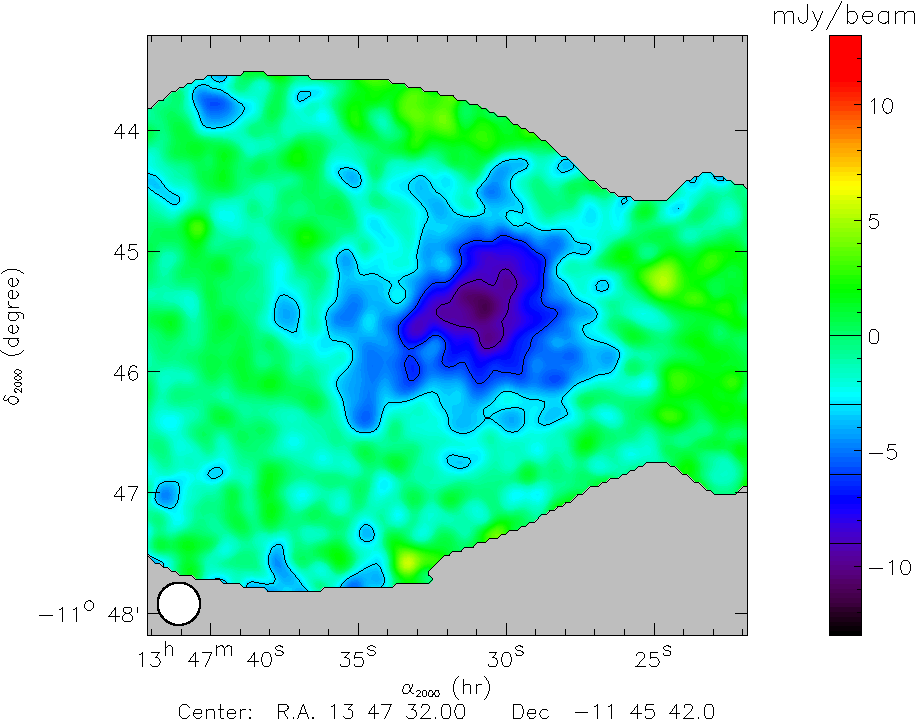
\includegraphics[width=0.3\textwidth]{./RXJ1347.pdf}   
\hfill
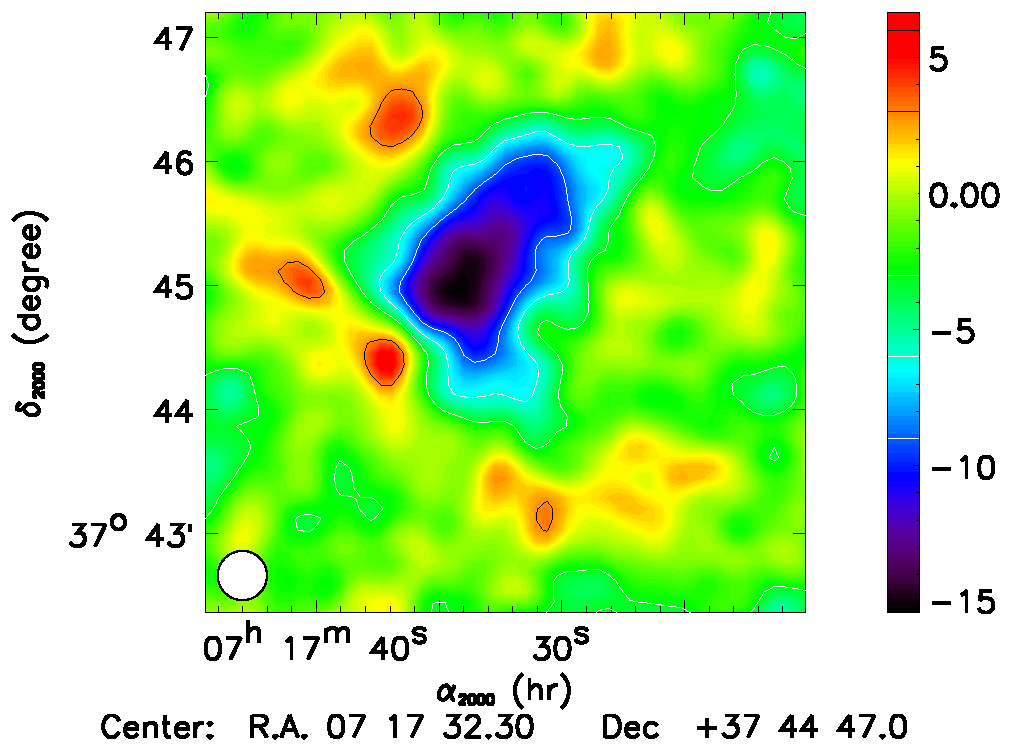
\includegraphics[width=0.32\textwidth]{./MACSJ0717_SZ.pdf}
\hfill
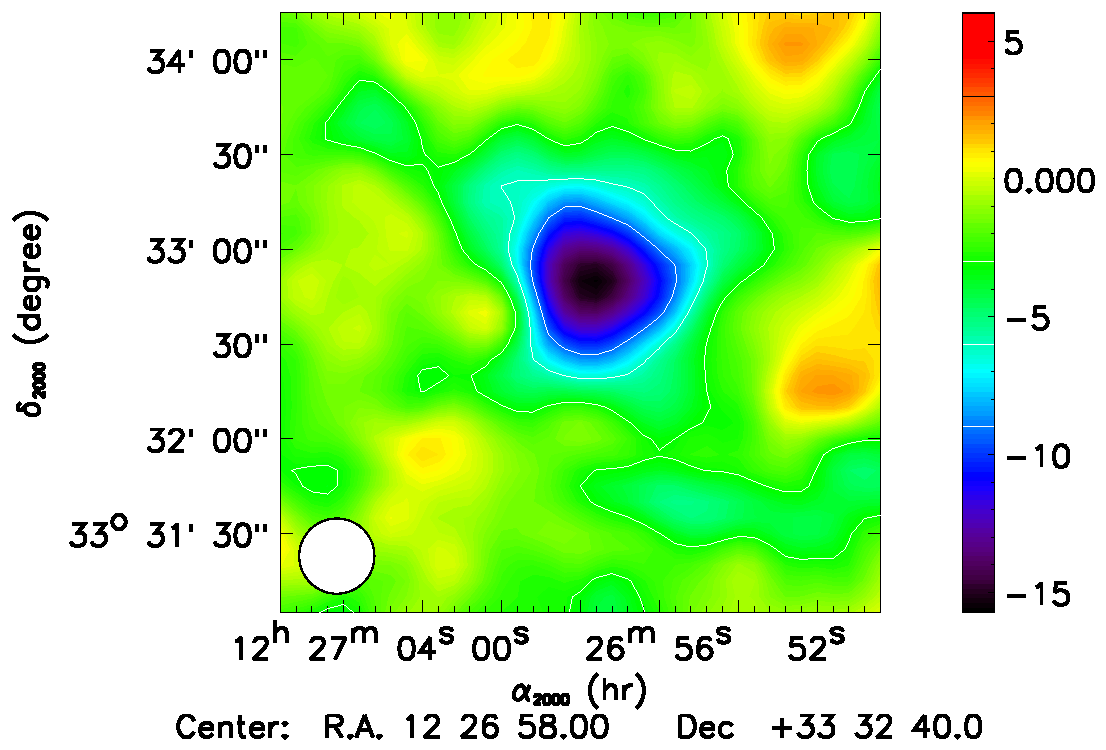
\includegraphics[width=0.35\textwidth]{./CLJ1227.pdf}   
\caption{\footnotesize Left -- 140 GHz flux density map of RX~J1347.5-1145, at z=0.45, observed during the technical run of 2012 \cite{adam2013}. This well known cluster is taken as a reference in order to estimate the expected flux intensity and distribution of the selected target.
Middle and right -- Preliminary signal to noise ratio maps of the clusters observed during the NIKA winter pool of February 2014. Left: MACS~J0717.5+3745 at z=0.55 is a triple merger, being one of the most disturbed cluster known. Right: CL~J1226.9+3332 at z=0.89 is a very distant cluster, it appears to be very compact but its core is known to be disturbed at scales smaller than the beam. These observations illustrate the power of NIKA for tSZ morphological studies. Note that for the moment only half of the data have been used for NIKA winter pool of February 2014 due to telescope antenna data issues that will be corrected soon.}
%\textcolor{red}{Faire le lien entre ces trios amas et les amas que l'on propose.}}
\label{fig:clusterRun8}
\end{figure}

\begin{figure}[h]
\centering	
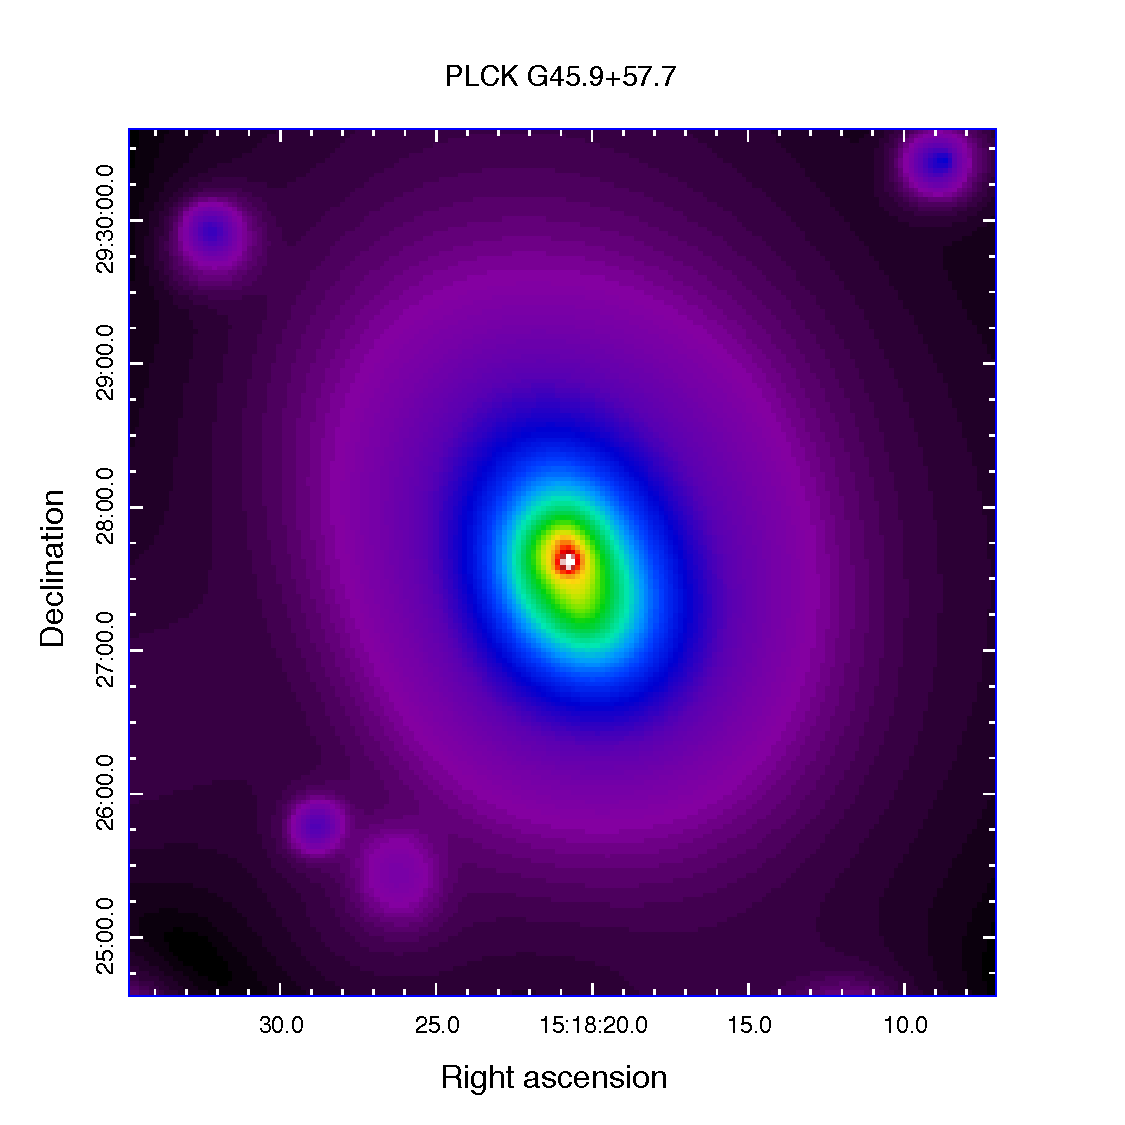
\includegraphics[width=0.45\textwidth]{./PSZ1G045_gwp.pdf}   
\hfill
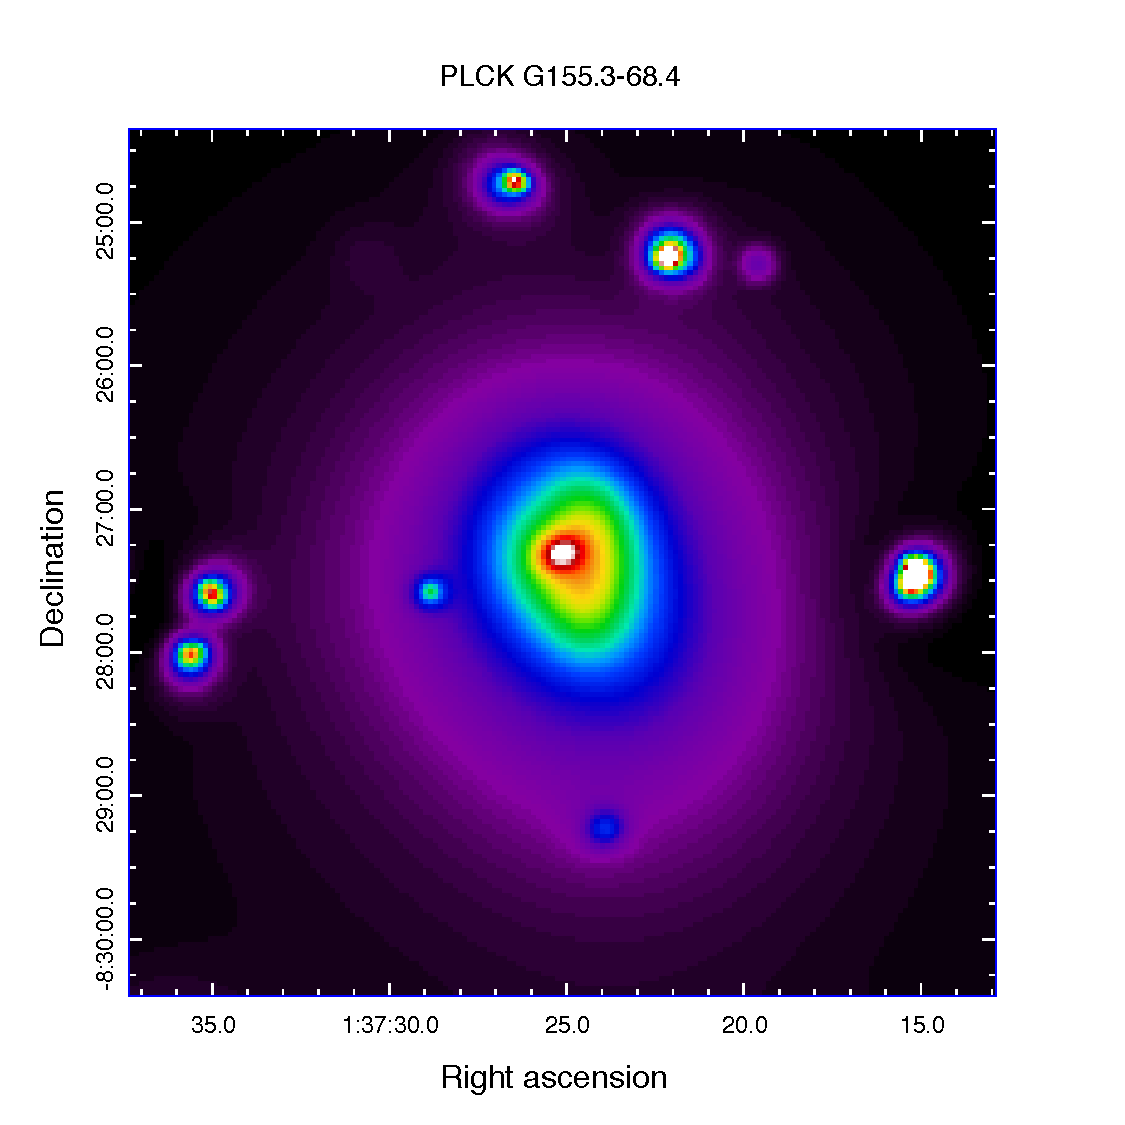
\includegraphics[width=0.45\textwidth]{./PSZ1G155_gwp.pdf}   
\hfill
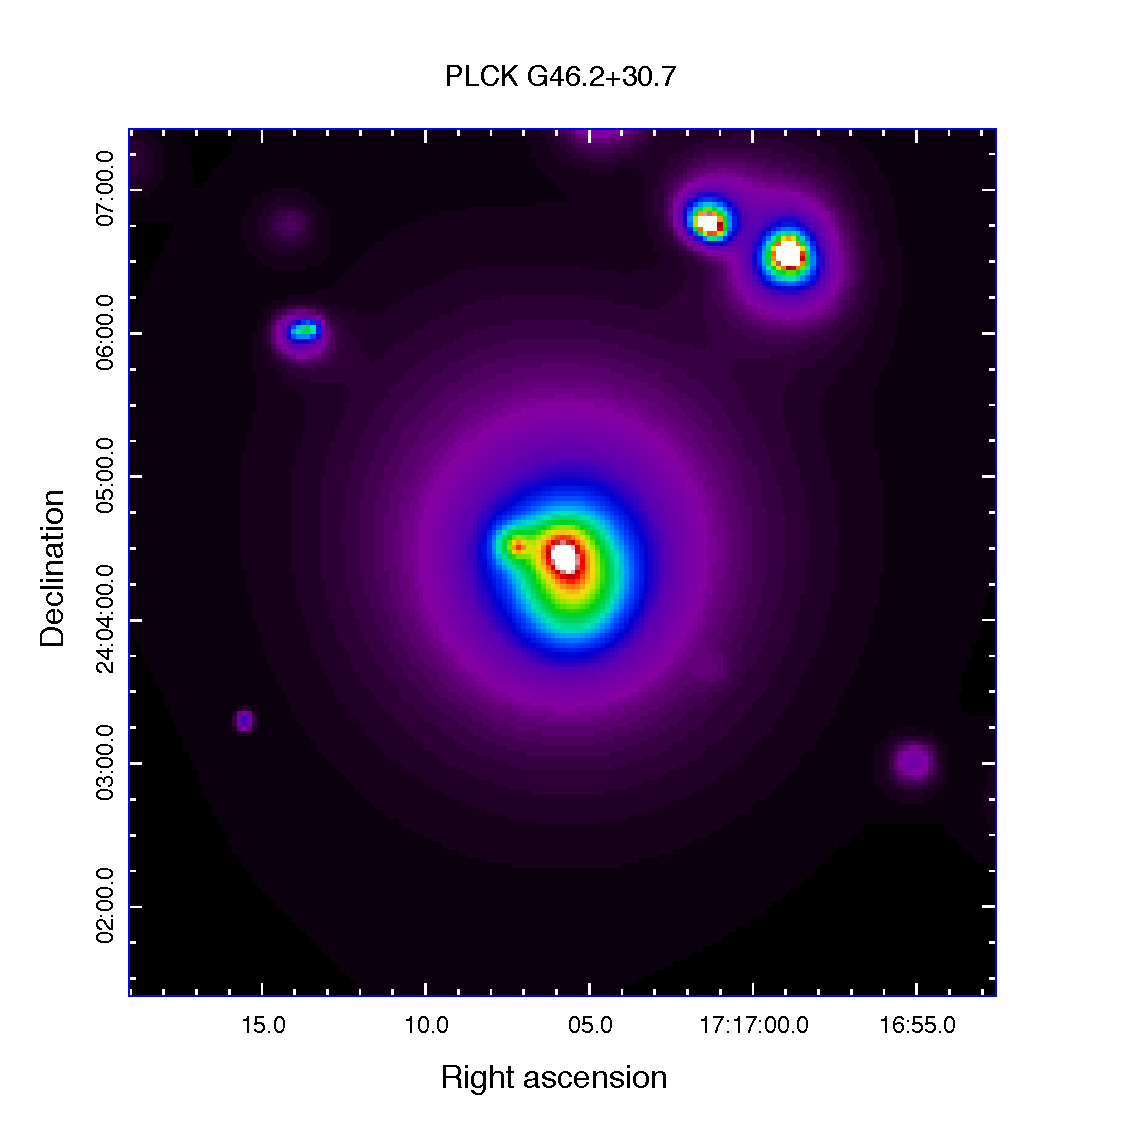
\includegraphics[width=0.45\textwidth]{./PSZ1G046_gwp.pdf}   
\hfill
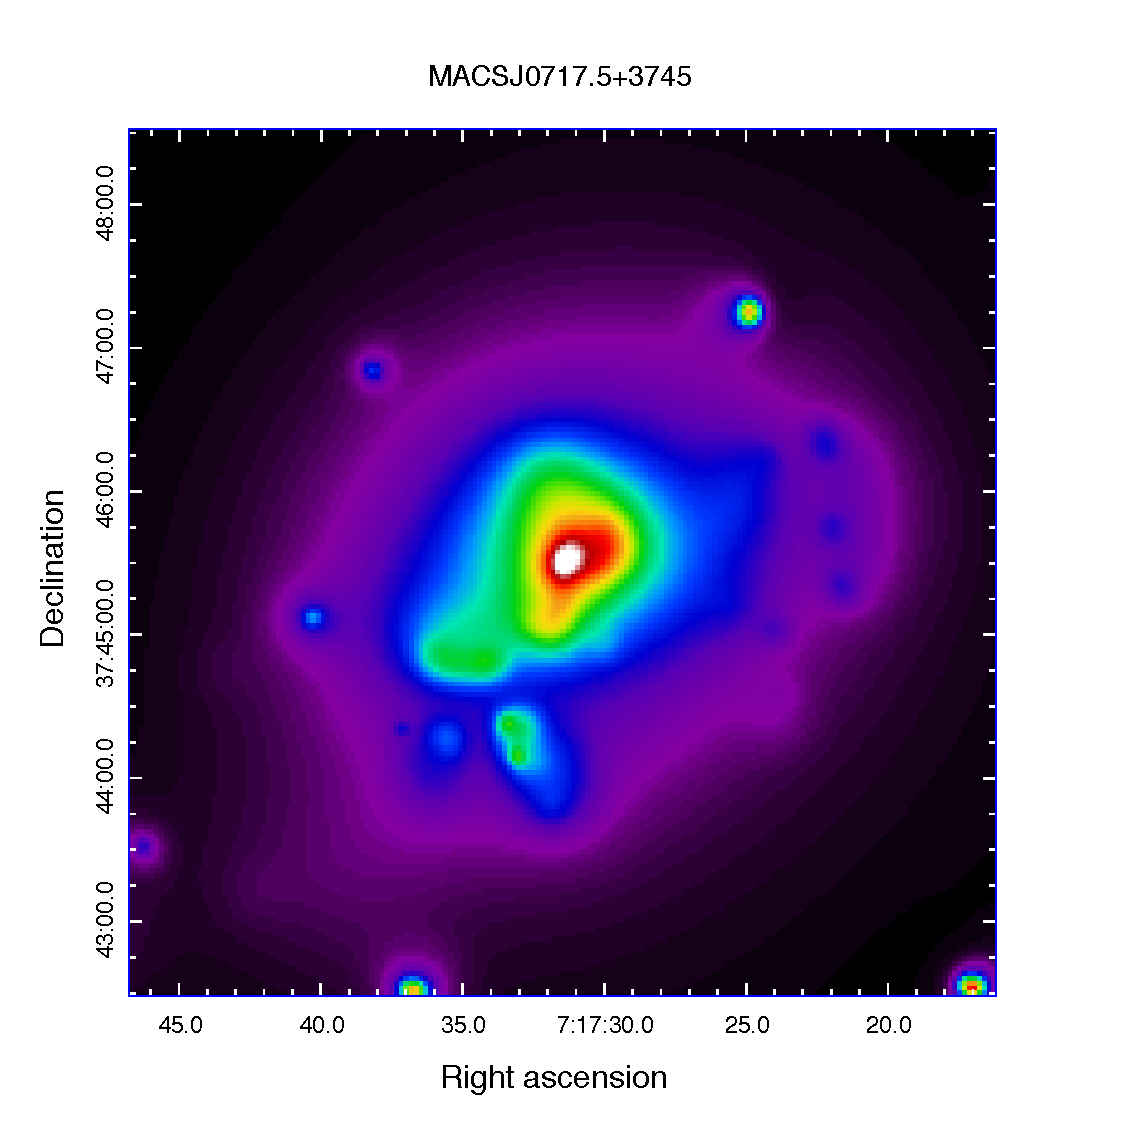
\includegraphics[width=0.45\textwidth]{./MACSJ0717_gwp.pdf}   
\caption{\footnotesize X-ray maps of the proposed clusters (top-left, top-right, bottom-left) and of MACS~J0717.5+3745 for reference (bottom-right). Image sizes are $6^\prime \times 6^\prime$. The three proposed clusters have centrally-peaked, circular X-ray morphologies, indicative of dynamical relaxation. MACS~J0717.5+3745 in contrast is highly disturbed in X-rays, as is also seen in the NIKA tSZ map (Fig.~\ref{fig:clusterRun8}, middle panel).}
%\textcolor{red}{and maybe the already observed cluster for reference? Is it possible to have these maps as proper pdf and with R.A-Dec. coordinates and typical frame size of 5-6 arcmin?}.}
\label{fig:xray}
\end{figure}


%-------------------------------------------------------------------
\begin{thebibliography}{9}

\bibitem[Adam et al.(2013)]{adam2013}
R. Adam, B. Comis, J.-F. Mac\'ias-P\'erez, {\it et al.} (2013) arXiv:1310.6237
  
  \bibitem[Basu et al.(2010)]{bas10}
  	K. Basu, Y.-Y. Zhang, M. Sommer et al. (2010), A\&A, 519, 29
  
    \bibitem[Billot et al.(2014)]{billot2014}
N. Billot, C. Kramer, S. Leclercq, {\it et al.} (2014), \\ http://www.iram.es/IRAMES/mainWiki/Continuum/TimeEstimatorScript

    \bibitem[Birkinshaw(1999)]{birkinshaw1999}
M. Birkinshaw (1999), Phys. Rep., 310, 97

    \bibitem[B\"{o}hringer \& Werner(2010)]{bohringer2010}
H. B\"{o}hringer \& N. Werner (2010), A\&A Rev., 18, 127

  \bibitem[Catalano et al.(2014)]{catalano2014}
A. Catalano, M. Calvo, N. Ponthieu, {\it et al.} (2014) arXiv:1402.0260
  
  \bibitem[Da Silva et al.(2004)]{das04}
  A.C. Da Silva, S.T. Kay, Liddle, A.R., \& Thomas, P.A. (2004), MNRAS, 348, 1401
  
  \bibitem[Komatsu et al.(1999)]{kom99}
  	E. Komatsu, H. Matsuo, T. Kitayama et al. (1999), ApJ, 516, L1
  
        \bibitem[Planck Collaboration I(2013)]{planck_overview2013}
Planck Collaboration I (2013) arXiv:1303.5062 

    \bibitem[Planck Collaboration XXIX(2013)]{planck_sz_cat2013}
Planck Collaboration XXIX (2013) arXiv:1303.5089 

      \bibitem[Planck Collaboration XXI(2013)]{planck_ymap2013}
Planck Collaboration XXI (2013) arXiv:1303.5081

      \bibitem[Planck Collaboration XX(2013)]{planck_cluster_count2013}
Planck Collaboration XX (2013) arXiv:1303.5080

	\bibitem[Pointecouteau et al.(1999)]{poi99}
		E. Pointecouteau, M. Giard, A. Benoit et al. (1999), ApJ, 519, L115

  \bibitem[Sunyaev \& Zeldovich(1972)]{sunyaev1972}
  R. A. Sunyaev, \& Y. B. Zel'dovich (1972), Astrophys. Space Phys. Res., 4, 173

  \bibitem[Sunyaev \& Zeldovich(1980)]{sunyaev1980}
    R. A. Sunyaev, \& Y. B. Zel'dovich (1980), ARA\&A, 18, 537
  
\end{thebibliography}

\end{document}
